\chapter{Project Development} \label{chap:implementation}

(...)\\

\section{Hypothesis}

(...)\\

\section{VESC Board}

The electric drive on which the motor controller is based is an open architecture project developed by the Swedish engineer Benjamin Vedder called VESC, which consists in the hardware design of a \ac{PCB} and the source code used to drive a \ac{BLDC} motor.\\

The VESC board was conceived and designed to be used in electric skateboards with the intention to create one of the best electronic speed controllers available. Since it was planned to be used in a skateboard, it has a small form-factor and it can be used for different applications with similar power demand. The hardware can also be modified by changing specific components to drive motors with higher power demand or by modifying the \ac{PCB} following the schematic design.

\begin{figure}[htbp]
\centering
\includegraphics[width=10cm]{Images/pcb_front.png} 
\caption[VESC Front Side]{Front Side of the VESC Board. The three wires at soldered at the right edge of the board are connected to the three phases of the brushless motor.}
\label{fig:pcb_front}
\end{figure}

The board consists of the following blocks, which will be explained in detail in this chapter:
\begin {enumerate}
	\item Power supply input
	\item Power MOSFETs three-phase inverter
	\item MOSFET driver
	\item Microcontroller unit
	\item Peripherals
	\begin {aenumerate}
		\item Temperature sensors
		\begin {aenumerate}
			\item Motor temperature sensor
			\item Board temperature sensor
		\end {aenumerate}
		\item Hall effect sensors
		\item RC Servomotor Output
		\item Debug LEDs
	\end {aenumerate}
	\item Communication interfaces
	\begin {aenumerate}
		\item USB
		\item CAN
		\item USART
		\item SPI
		\item I2C
	\end {aenumerate}
\end {enumerate}

\subsection{Power Supply Input}
The power is supplied into the board by means of soldering 2 wires into large pads placed closely to the three-phase inverter nodes $V\_SUPPLY$ and $GND$. $V\_SUPPLY$ and $GND$ are the positive and negative nodes of the power supply source respectively. The power is supplied from a power regulator for static applications or from a battery for mobile applications, like in the case of ROBI'. It is also specified that there should be a decoupling capacitor connected in parallel to the power supply port.

\begin{figure}[htbp]
\centering
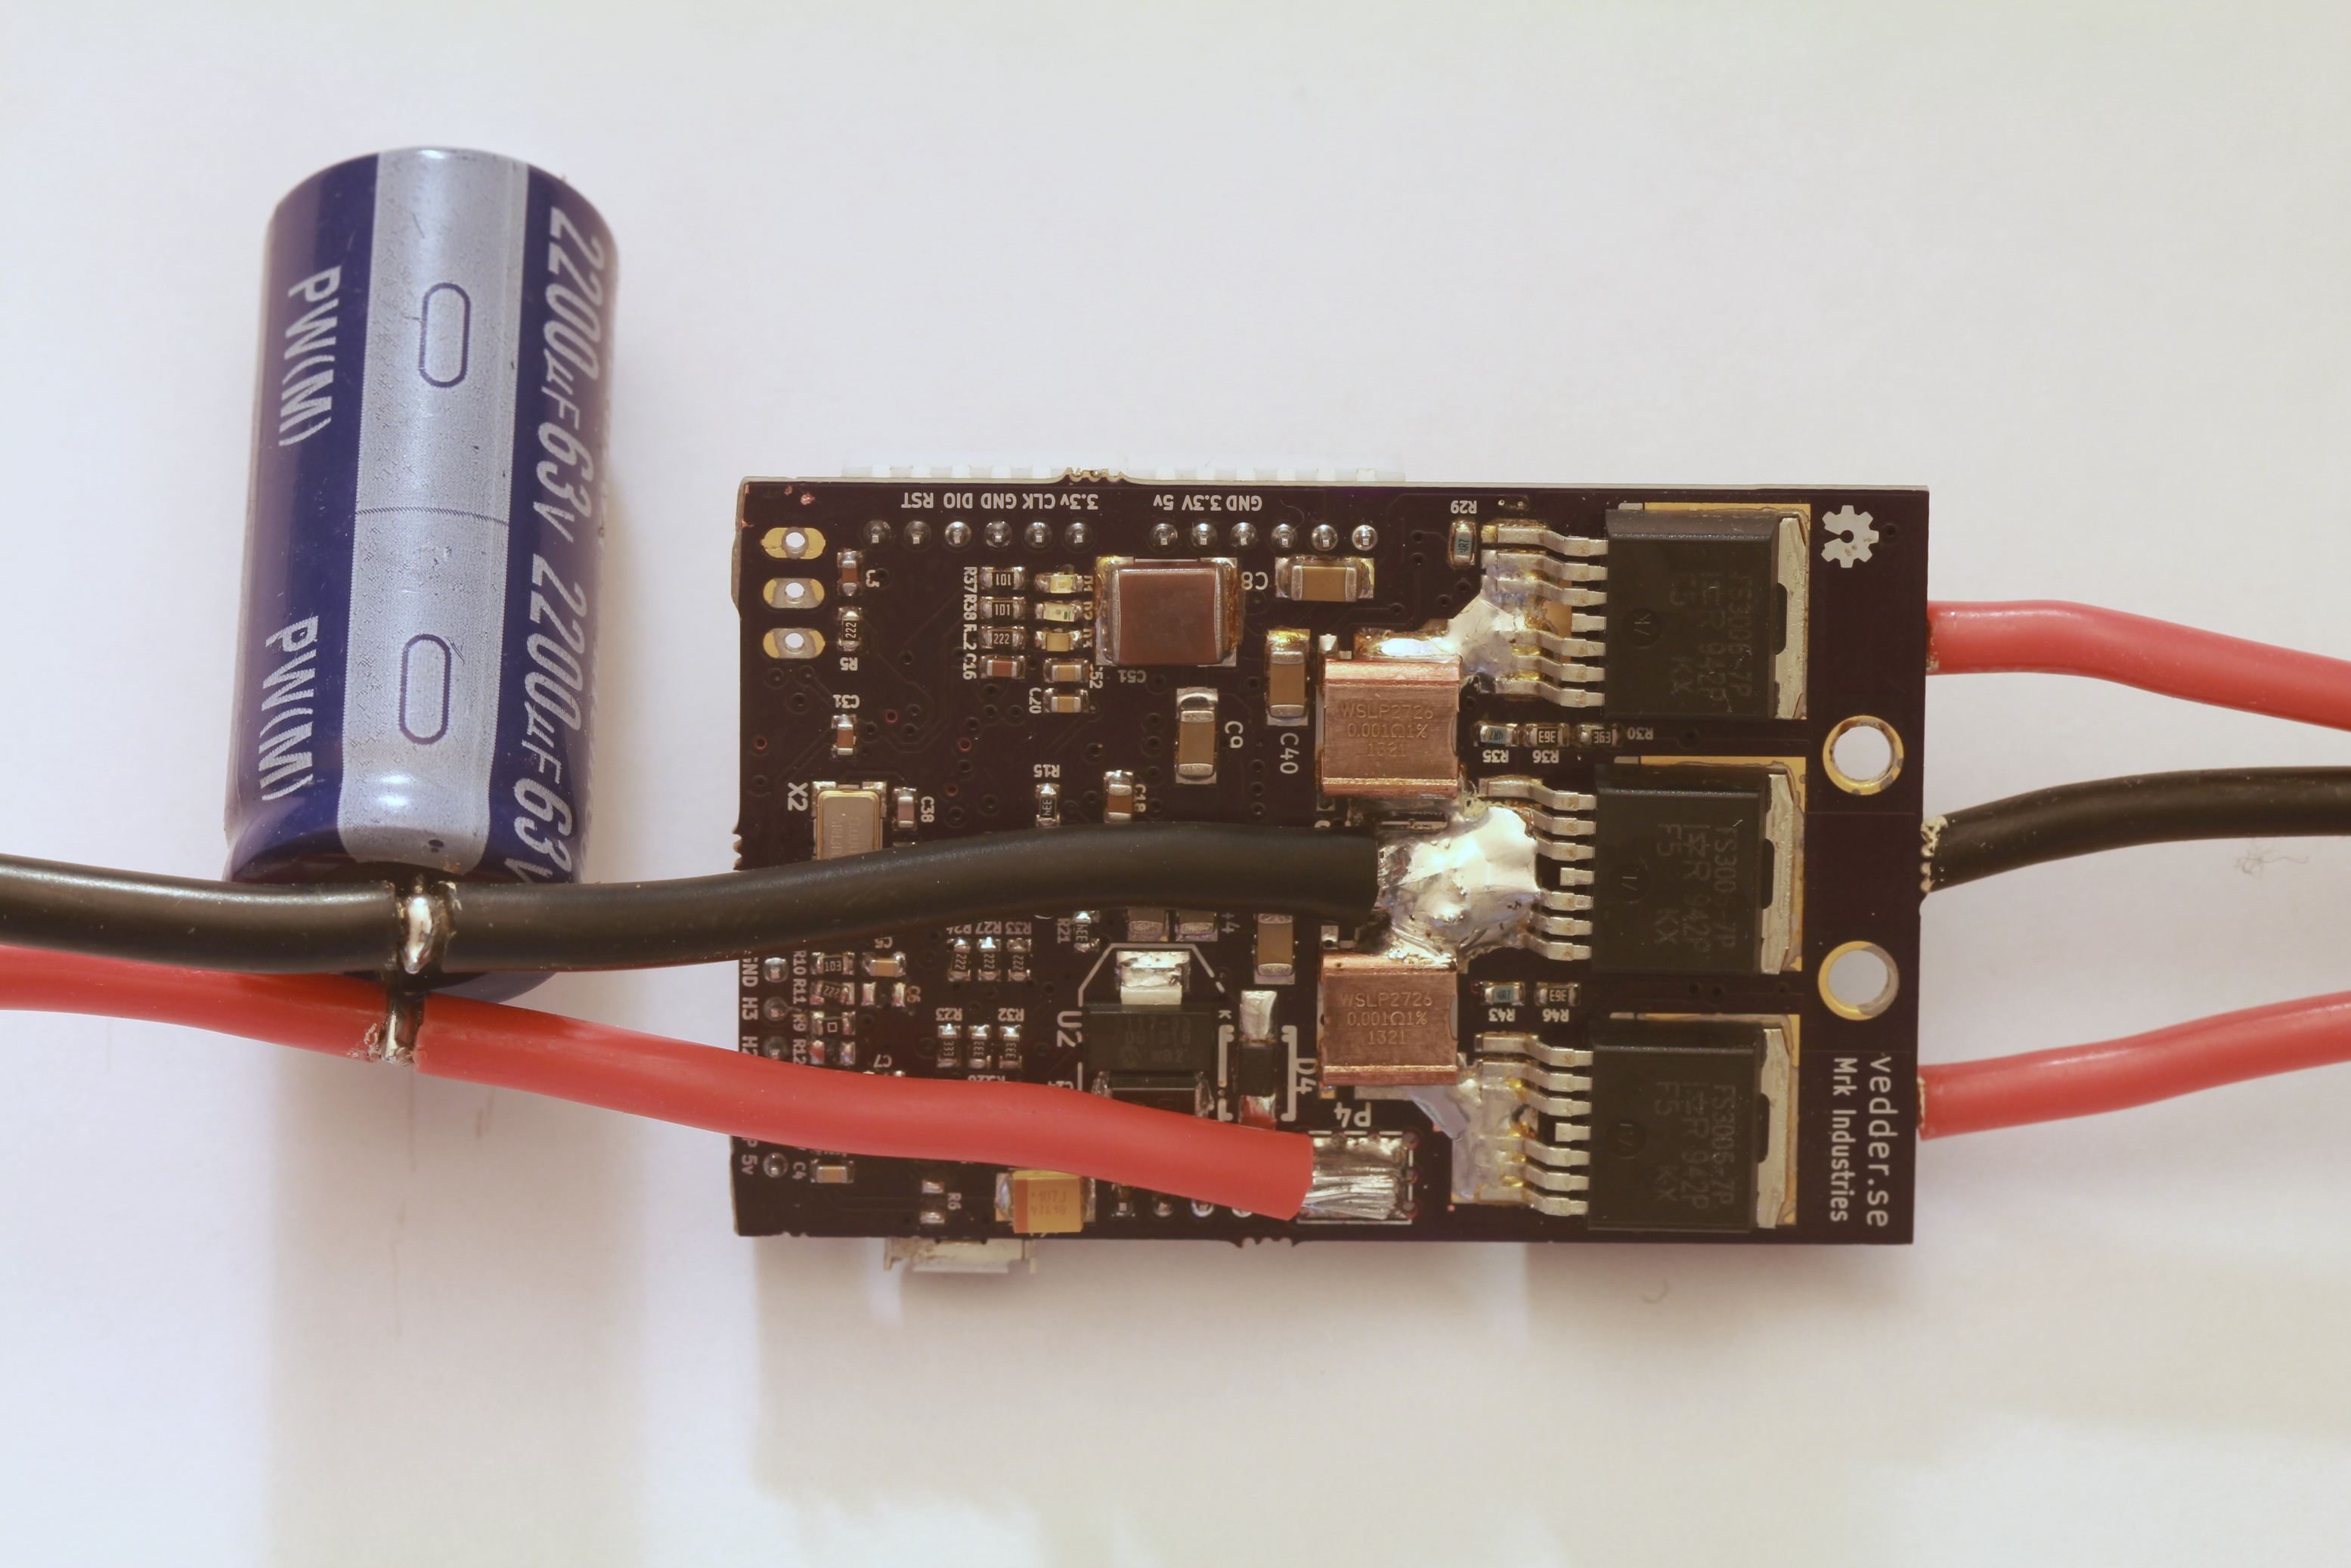
\includegraphics[width=10cm]{Images/pcb_back.png} 
\caption[VESC Back Side]{Back Side of the VESC board. The red and black wires are the power supply input $V\_SUPPLY$ and $GND$ respectively.}
\label{fig:pcb_back}
\end{figure}

\subsubsection{Power Supply Range}

The voltage range of the VESC board is defined by the \ac{MOSFET} driver integrated circuit DRV8302, which specifies an operating supply voltage range from $8V$ to $60V$, but allows a maximum voltage supply up to $65V$ \ref{DRV8302}. All the other components of the board, mainly capacitors and power \ac{MOSFET}s, must be selected according to this voltage range.

The current range of the board is limited by the \ac{MOSFET}s current limit and by the width of the traces in the \ac{PCB}. This maximum values will be addressed later in the section dedicated to the power \ac{MOSFET}s used in the board.

%INCLUDE TABLE WITH ABSOLUTE VALUES

\subsubsection{Bulk Electrolytic Capacitor}

It is important to place a bulk capacitance with an appropiate capacitance value and voltage range in parallel to the input of the power supply of a motor drive system. The main objective of a bulk capacitance is to control the voltage deviation at the input of a system when the converter is responding to an output load transient, meaning that if there is a load increase and the power supply is not able to provide the current instantaneously for the motor, the current must be provided by the bulk capacitor. The higher the capacitance at the input of the system, the lower the deviation at the load, but this comes at a cost of price and space, since the capacitance value of a capacitor is proportional to the size of its parallel plates. The value of the input bulk capacitor is determined mainly by the following factors:

\begin {enumerate}
	\item The largest amount of current required by the motor
	\item The capacitance of the power supply and its ability to source current
	\item The parasitic inductance between the power supply and the motor
	\item The acceptable voltage ripple
	\item The type of motor
\end {enumerate}

The datasheet of a motor driver should generally provide a recommended value for the bulk capacitor, but it is necessary to calculate and test the value to determine if it's appropiate. The voltage rating of a bulk capacitor must be higher than the value of the power supply to provide a margin for cases in which the motor transfers energy to the supply, which would increase its voltage and would damage a capacitor with a smaller value than the resulting voltage.

The magnitude of the input transient is calculated as following:

\begin{equation} \label{current_ripple}
	\Delta I_{in} = \frac{V_{out}}{V_{in}\eta}\cdot \Delta I_{out}
\end{equation}

where $\eta$ is efficiency, $\Delta I_{out}$ is the output transient current, $\Delta I_{in}$ is the input transient current, $V_{out}$ is the nominal output voltage and $V_{in}$ is the nominal input voltage. After determining the input transient, we can calculate the capacitance value by using the following formula:

\begin{equation} \label{current_ripple_2}
	C = \frac{1.21 \cdot I_{tr}^{2} \cdot L}{\Delta V^{2}}
\end{equation}

%[http://www.ti.com/lit/an/slta055/slta055.pdf]
%[http://www.analog.com/media/en/training-seminars/tutorials/MT-101.pdf]


Since there is no filtering inductance in the system, we can consider a stray inductance of 50 nH in the calculation. If we consider a transient current $I_{tr}$ equal to the rated current of the in-wheel motor, $14 A$ approximatedly, and a voltage ripple of $100 mV$, we obtain a capacitance value of $1185.8\mu F$ for the bulk capacitance. By looking for commercially available capacitor values, we can increase the value of the capacitor to 2200uF and, considering the maximum input voltage value of the motors, we need double that value and define a voltage range of $70V$, which is a commercially available value for a capacitor.

The voltage of the capacitor is chosen double of the rated voltage of the motor because it is possible that, when the motor enters a braking mode, the energised coils apply a voltage equal to the \ac{BEMF} and the voltage bus $V_{DC}$ increases up to $2\cdot V_{DC}$.

It is important to note that since the value of this capacitance is large, also its size will be large, therefore it's important to consider its dimensions to setup a mechanically stable position for such capacitance with aims of avoiding hardware malfunction.

\subsubsection{Power Supply Wiring}

The strategy of soldering the wires directly to the pads in the \ac{PCB} helps reduce the size and price of the board since it avoids the use of large power traces in that would be needed if a regular receptacle connector was to be used.

Anyway, the practice of soldering a wire directly to a \ac{PCB} is discouraged mainly in circuits that will be mounted in a system designed to be in movement (i.e. automotive or aerospace applications) because the wire used in these applications is made of delicate copper strands which can break easily with movement of the board or of the wires and cause a short circuit or a loose contact, both of which might lead to catastrophic failures , so there is a risk in this board since it will be mounted in systems that will be in constant movement. Since this board was designed this way to reduce space consumption, the trade-off between safety and size was balanced into the size constraints, therefore some cautions must be taken to avoid problems, mainly because these wires carry a considerable amount of current and they pass over many components of the board as seen in Figure \ref{fig:pcb_back}.

%(https://electronics.stackexchange.com/questions/129907/what-is-the-best-way-to-solder-these-wires-to-circuit-board)
%(http://uk.rs-online.com/web/generalDisplay.html?id=solutions/pcb-connectors)

The first consideration to be made is the wire gauge and insulation type. The wire gauge is a measurement of the wire diameter, which determines the amount of electric current that a wire can safely carry, as well as its electrical resistance and weight. Since the wire has an implicit resistance depending on its diameter as stated by Pouillet's Law:

%(http://en.wikipedia.org/wiki/Wire_gauge)

\begin{equation} \label{pouillet}
	R = \frac{\rho L}{A}
\end{equation}

where $\rho$ is the electrical resistivity of the material, $L$ is the length of the wire and $A$ is the cross-sectional area of the wire, there is also a voltage drop in the transmission line depending on the current flowing through the wire. This voltage drop can be neglected or not depending on the length of the wire being used, which defines 2 types of wiring: chassis wiring and transmission line wiring. For this board, it is suggested to use short wires to avoid a large voltage drop and to ease the handling of such wire until it reaches the output of the enclosure that will protect the circuit. In either case, the wire can be considered as chassis wiring since a transmission line wiring is considered for wires larger than 2 meters.

%(https://en.wikipedia.org/wiki/Electrical_resistivity_and_conductivity)

The second consideration regarding the wire selection is the insulation material. Since the current passing through the copper also implies power consumption due to the resistance of the copper, there is heat transfer from the wire to its surroundings. To protect the copper strands from its surroundings and vice versa, wires are covered by an insulating material, which has low thermal and electrical conductivity.

Since the heat exchange calculation of the wire would require many assumptions, it’s a normal practice to select the type of wire using tables that consider the temperature rise in the wire according to different currents and lengths. In the case of the \ac{PMSM} motor used in ROBI', the maximum steady state current would be approximately $14A$, therefore we can use a table of wire gauges and currents under (…) 

%(https://www.powerstream.com/Wire_Size.htm)

%RESULT OF THE CALCULATION\\

\subsection{Power MOSFET Three-Phase Inverter}
The three-phase inverter used in the VESC board is based on the power \ac{MOSFET} IRFS7530-7PPbF, manufactured by the semiconductor company International Rectifier.

\begin{figure}[htbp]
\centering
\includegraphics[width=10cm]{Images/inverter_3.png} 
\caption[VESC Board Inverter]{Three-phase inverter implemented using power MOSFETs.}
\label{fig:inverter_3}
\end{figure}

This \ac{MOSFET} is based on the HEXFET Power \ac{MOSFET} technology, which is a Vertical Double-diffused MOS transistor (VDMOS) with hexagonal elementary cells in parallel which maximizes the $W/L$ ratio of the transistor, reducing its on-resistance $R_{DS(ON)}$. 
%(ref to Gionni and the datasheet).\\

\begin{figure}[htbp]
\centering
\includegraphics[width=10cm]{Images/irf.png} 
\caption[IRF 1]{...}
\label{fig:irf}
\end{figure}

\begin{figure}[htbp]
\centering
\includegraphics[width=10cm]{Images/irf_2.png} 
\caption[IRF 2]{...}
\label{fig:irf_2}
\end{figure}

\subsubsection{Switching Times}

%(...)\\


\subsection{MOSFET Driver}

The central component in the VESC board around which the rest of the circuit was designed is the integrated circuit $DRV8302$, a brushless motor inverter driver manufactured by Texas Instruments.

%INCLUDE SIMPLIFIED SCHEMATIC DIAGRAM OF THE DRIVER\\

The DRV8302 provides three half bridge drivers capable of driving two N-channel MOSFETs each. (...)

The device supports up to 1.7-A source and 2.3-A peak current capability. (...)

The DRV8302 can operate off of a single power supply with a wide range from 8-V to 60-V. (...)

It uses a bootstrap gate driver architecture with trickle charge circuitry to support 100 duty cycle. (...)

The DRV8302 uses automatic hand shaking when the high side or low side MOSFET is switching to prevent current shoot through. (...)

Integrated VDS sensing of the high and low side MOSFETs is used to protect the external power stage against overcurrent conditions. (...)

The DRV8303 includes two current shunt amplifiers for accurate current measurement. The amplifiers support bi-directional current sensing and provide and adjustable output offset up to 3 V. (...)

The DRV8302 also includes an integrated switching mode buck converter with adjustable output and switching frequency. The buck converter can provide up to 1.5 A to support MCU or additional system power needs. (...)

A hardware interface allows for configuring various device parameters including dead time, overcurrent, PWM mode, and amplifier settings. Error conditions are reported through the nFAULT and nOCTW pins. 3.3-V and 5-V Interface Support. (...)


\subsection{Microcontroller Unit}

The processor for which this board was designed is the STM32F405rg: a 64-pin IC microcontroller of the STMicroelectronics family of 32-bit devices with an ARM Cortex-M4 CPU and a core operating frequency up to 168 MHz. The Cortex-M4 core features a \acf{FPU} single precision which supports all ARM single-precision data-processing instructions and data types. It also implements a full set of \acf{DSP} instructions, which makes it ideal for the signal processing required to drive \ac{PMAC} motors. This microcontroller also includes three 12-bit \ac{ADC}s and supports USART, I2C, SPI, USB and CAN communication interfaces, improving the versatility of the VESC board. The memory of the microcontroller consists in 1024 kB of Flash memory and 192 kB of SRAM memory.


\subsection{PCB Layout}

(...)\\


\section{Measurement Board}

(...)\\

\subsection{Voltage Measurement}

(...)\\

\subsection{Current Measurement}

(...)\\

\subsection{Data acquisition}
usb
(...)\\

\section{Angular Position Sensor}

(...)\\

\section{Miosix}

(...)\\

\section{Test Setup}

(...)\\

\subsection{Robi Setup}

(...)\\

\subsubsection{Marelli Generator as Load}

(...)\\

\section{Algorithms Implementation}

(...)\\

\subsection{6-Step Drive Implementation}

(...)\\

\subsection{Field Oriented Control Implementation}

(...)\\






